\def\ind[#1]{\mathbb{I}_{#1}}
\def\extendedreal{\bar{\mathbb{R}}}
\def\hsetover[#1]{\mathbb{Z}^{#1}}

\chapter{Integration III} \label{integration}
\doublespacing

``Chapter goals''

Section 4.1 will cover a conventional treatment of the Lebesgue integral, for those already familiar with the construction, this may be skipped. 

%%%%%%%%%%%%%%%%%%%%%%%%%%%%%%%%%%%%%%%%%
%
% LEBESGUE INTEGRATION
%
%%%%%%%%%%%%%%%%%%%%%%%%%%%%%%%%%%%%%%%%%

\section{Sigma Algebras}

Before we can talk about the Lebesgue integral we must first set the stage, so to speak.



\begin{definition}
Let $X$ be a non-empty set. A \textbf{$\sigma$-algebra on the set $X$}, $\Sigma$,  is a family of subsets of $X$ such that:
\begin{enumerate}
\item $\Sigma$ is non-empty
\item \emph{Closed under complement.} If $E \in \Sigma$, then $X \setminus E \in \Sigma$.
\item \emph{Closed under countable union.} If $E_1, E_2, ... \in \Sigma$ then $(E_1 \cup E_2 \cup ... ) \in \Sigma$.
\end{enumerate}
The pair $(X, \Sigma)$ is called a \textbf{measurable space} and elements of $\Sigma$ are called the \textbf{measurable sets} (of $X$).
\end{definition}

It can easily be shown through the use of De Morgan's laws that a $\sigma$-algebra is also closed under countable intersection as well.
\begin{example}
$\{ \emptyset, X \}$ is a $\sigma$-algebra on $X$. In fact, $X$ and $\emptyset$ are members of \emph{every} $\sigma$-algebra on $X$.
\end{example}

\begin{example}
$2^X$ is a $\sigma$-algebra on $X$.
\end{example}

However, we would also like to be able to construct more interesting $\sigma$-algebras.

\begin{definition}
Given an arbitrary family of subsets $F \subseteq 2^X$, there is a unique smallest $\sigma$-algebra containing $F$ which is called the \textbf{$\mathbf{\sigma}$-algebra generated by $F$} and we will denote as $\sigma(F)$.
\end{definition}

Can be constructed by taking the intersection of all $\sigma$-algebras containing $F$.

Of particular interest to us is the $\sigma$-algebra generated by a topology, $\mathcal{T}(X)$. 

Borel $\sigma$-algebra: $\mathcal{B}(X) = \sigma(\mathcal{T}(X))$

\section{The Lebesgue Integral}

\begin{definition}
Let $(X, \mu )$ be a measure space and $S \in \mathcal{L}(X, \mu)$ a measurable set. If $\ind[S]$ is indicator function $\ind[S] : X \to \{ 0, 1 \}$ given by $\ind[S] (x) = 1$ if $x \in S$ and $\ind[S] (x) = 0$ otherwise.
Then we define:
\begin{equation}
\int_X \! \ind[S] \; d \mu := \mu ( S )
\end{equation}
\end{definition}

We define a simple function as a function which maps to a finite set.
\begin{theorem}
If $\varphi$ is a simple function, then we it can be represented as a finite sum of indicator functions:
\begin{equation}
\varphi := \sum_{k=0}^n a_k \ind[E_k]
\end{equation}
Where $\{ a_k \}_{k=0}^n$ is the set of values in the range of $\varphi$ and $E_k = \varphi^{-1}( \{ a_k \} )$, the set of all points which map to $a_k$.
\end{theorem}

This allows us to define the integral of a simple function.

\begin{definition}
Let $\varphi = \sum_{k=0}^n a_k \ind[E_k]$ be a simple function. We define the integral:
\begin{equation}
\int_X \! \varphi \; d \mu = \int_X \! \sum_{k=0}^n a_k \ind[E_k] d \mu = \sum_{k=0}^n a_k  \int_X \! \ind[E_k] d \mu
\end{equation}
\end{definition}

Next we define integral of a non negative functions in $\extendedreal$

\begin{definition}
Let $(X,\mu)$ be a measure space and $f: X \to [0,\infty]$. 
\begin{equation}
\int_X \! f \; d\mu := \text{sup} \left\{ \int_X \varphi : \varphi \text{ simple, and } 0 \leq \varphi \leq f \right\}
\end{equation}
\end{definition}

We use the simple function $\psi_n$ defined as:
\begin{equation}
\psi_n = \sum_{k=0}^{n2^n -1} \left[ \left(\frac{k}{2^n}\right)^{\left[ \frac{k}{2^n}, \frac{k+1}{2^n} \right)} \right] + n^{[n,\infty]}
\end{equation}

Notationally, this definition is rather heavy but is easily understood geometrically as seen in Figure 4.1

\todo{figure description}
\begin{figure}
\caption[Approximations using simple functions]{asdfasdf }
\centering

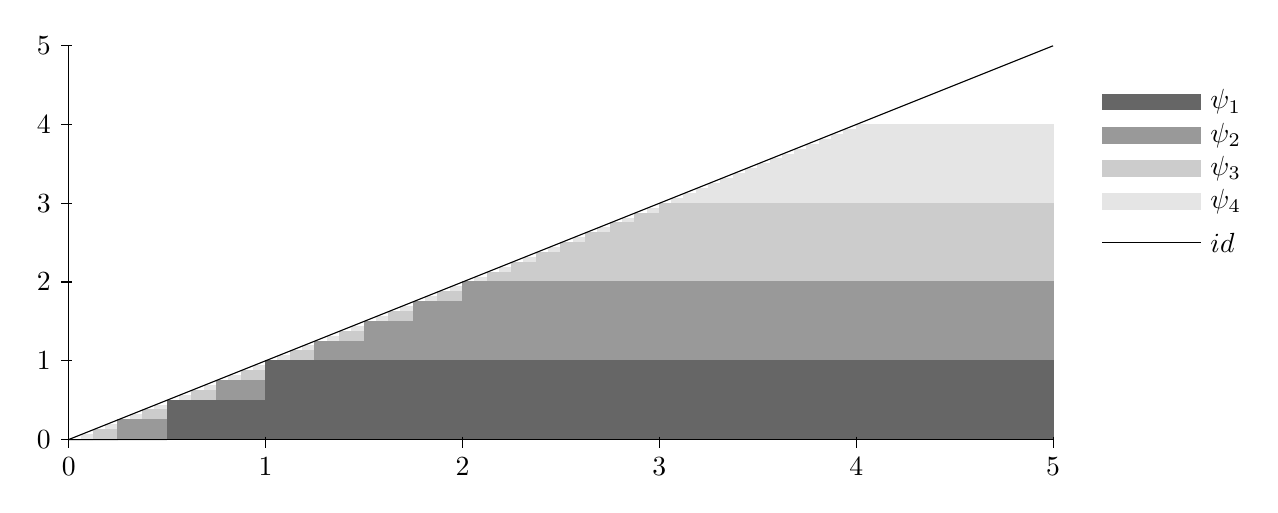
\begin{tikzpicture}[y=1cm, x=2.5cm]


	\foreach \x in {0,0.0625,...,3.99}
		\draw[fill, color=black!10] (\x,0) rectangle ++ (0.0625, \x);
	\draw[fill, color=black!10] (4,0) rectangle (5,4);

	\foreach \x in {0,0.125,...,2.9}
		\draw[fill, color=black!20] (\x,0) rectangle ++ (0.125, \x);
	\draw[fill, color=black!20] (3,0) rectangle (5,3);
	
	\foreach \x in {0,0.25,...,1.9}
		\draw[fill, color=black!40] (\x,0) rectangle ++ (0.25, \x);
	\draw[fill, color=black!40] (2,0) rectangle (5,2);
	
	\foreach \x in {0,0.5,...,0.9}
		\draw[fill, color=black!60] (\x,0) rectangle ++ (0.5, \x);
	\draw[fill, color=black!60] (1,0) rectangle (5,1);
	
	
	
 	%axis
	\draw(0,0) -- coordinate (x axis mid) (5,0);
    	\draw (0,0) -- coordinate (y axis mid) (0,5);
    	%ticks
    	\foreach \x in {0,1,...,5}
     		\draw (\x,1pt) -- (\x,-3pt)
			node[anchor=north] {\x};
    	\foreach \y in {0,1,...,5}
     		\draw (1pt,\y) -- (-3pt,\y) 
     			node[anchor=east] {\y}; 
	
	\draw (0,0) -- (5,5);

	
	%legend
	\begin{scope}[shift={(5.25,2.5)}] 
	
	\draw[yshift=4\baselineskip, fill, color=black!60] (0,0) rectangle (0.5,0.2) --++ (0,-0.1)
		node[right, color=black]{$\psi_1$};
	\draw[yshift=3\baselineskip, fill, color=black!40] (0,0) rectangle (0.5,0.2) --++ (0,-0.1) 
		node[right, color=black]{$\psi_2$};	
	\draw[yshift=2\baselineskip, fill, color=black!20] (0,0) rectangle (0.5,0.2) --++ (0,-0.1) 
		node[right, color=black]{$\psi_3$};
	\draw[yshift=\baselineskip, fill, color=black!10] (0,0) rectangle (0.5,0.2) --++ (0,-0.1) 
		node[right, color=black]{$\psi_4$};
	\draw (0,0) -- (0.5,0) node[right] {$id$};
	\end{scope}
\end{tikzpicture}
\end{figure}


Which for any non-negative $f$ allows us to define $\varphi_n = \psi_n \circ f$ a simple function.

Obviously we have $\varphi_n$ simple since $\psi_n$ is simple. 

Since $\psi_n(x) \leq x$ for all $x$ then we also have $0 \leq \varphi_n \leq f$.

Most importantly we have $0 \leq f(x) - \varphi_n(x) \leq 2^{-n}$ and so $\varphi_n$, uniformly approaches $f$ as $n$ approaches infinity. 

\begin{theorem}
Let $f$ be a function mapping to $\mathbb{R}$. Then $f = f^+ - f^-$ where $f^+$ and $f^-$ are non-negative functions given by:
\begin{align}
f^+(x) &:= \mathrm{max}( 0, f(x)) \\
f^-(x) &:= \mathrm{max}(0, -f(x)) 
\end{align}
\end{theorem}

Now we have everything we need to define integrals for arbritrary functions mapping to $\mathbb{R}$:

\begin{definition}
asdfasd
\begin{equation}
\int_X f d \mu = \int_X f^+ d \mu - \int_X f^- d \mu
\end{equation}
\end{definition}

%\begin{example}
%\begin{equation}
%\int_{[0,1]} \! \ind[\mathbb{Q}] \; d\mu = \mu(\mathbb{Q}) = 0
%\end{equation}
%\end{example}

%\begin{example}
%\begin{equation}
%\int_{[0,1]} \! x^2 d \mu = \lim_{n \to \infty} \sum_{k=0}^{2^n -1} \frac{k}{2^n} \int_{[0,1]} \ind[[k/2^n, (k+1)/2^n)]
%\end{equation}
%\end{example}

This was a standard treatment of Lebesgue integration.

Mathematically it is very simple to extend this to integrals of hybrid sets over $L(X, \mu)$ by linearity.
That is, given $\Gamma \in \hsetover[\mathcal{L}(X,\mu)]$:

\begin{equation}
\int_\Gamma f d \mu = \sum_{\sigma \in \Gamma} \Gamma(\sigma) \int_\sigma f d\mu
\end{equation}
